\section{Schema Hierarchies}

EL schemas support two hierarchical organizations of schemas.
In the \textbf{specialization} hierarchy, a child schema inherits the semantics of a parent schema, and may then further restrict the set of participants, their types and relationships, and the events; this hierarchy is comparable to an object-oriented ontology.
In the \textbf{compositional} hierarchy, a child schema is \textit{embedded} as a step in a parent schema; it is represented in the parent's \texttt{:Steps} section as its header formula, but can be ``expanded'' to reveal its full semantics, which include its own steps, participants, and nested schemas.

\subsection{Compositional Hierarchy}
\begin{figure}
    \centering
    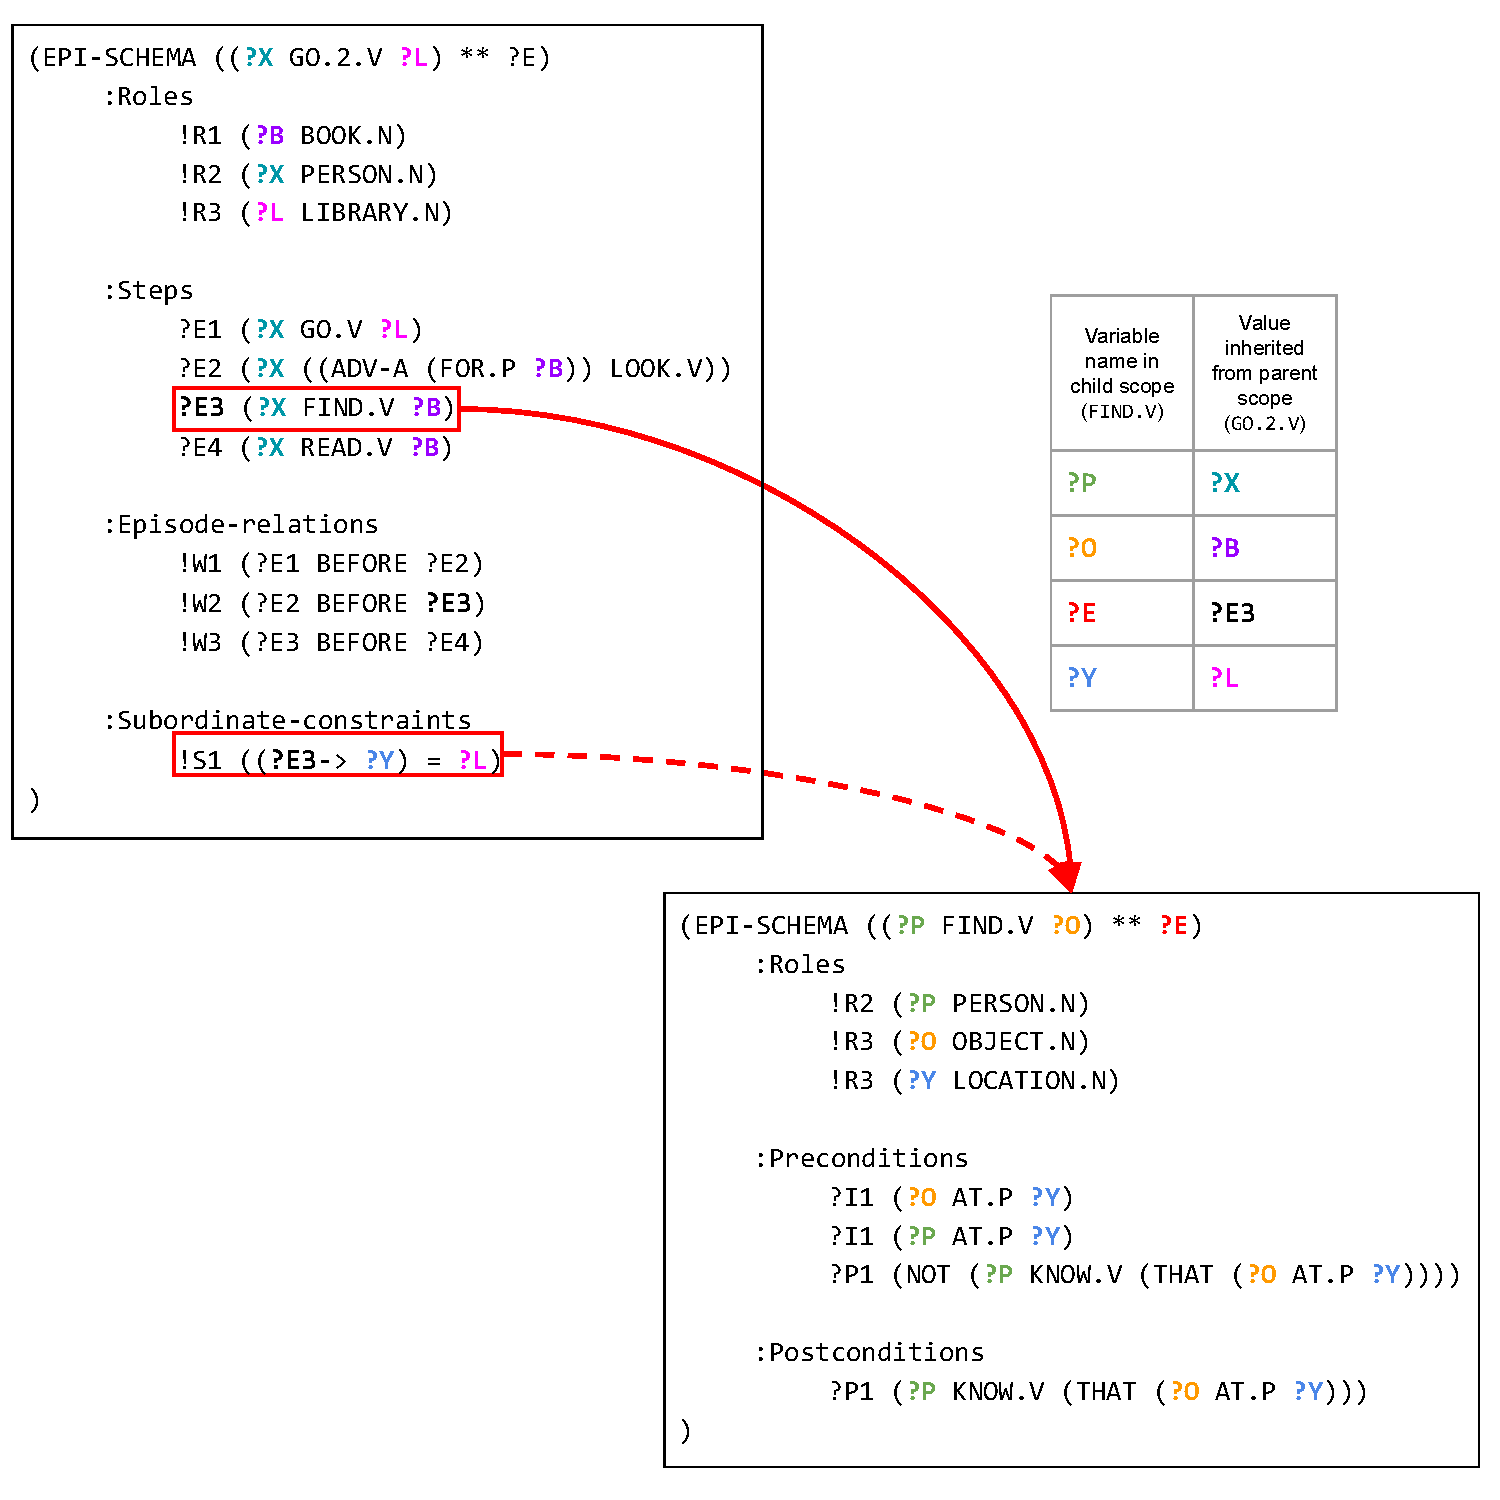
\includegraphics[width=\columnwidth]{CH3_schemas/nesting}
    \caption{An illustration of the \textbf{compositional} hierarchy, in which a \textit{child} schema nested within a \textit{parent}. The child schema \texttt{FIND.V}, shown in the bottom right, is nested within the parent schema \texttt{GO.2.V}, shown in the top left. A table in the upper right shows the new values for the child schema's variables, each inherited from the parent schema.}
    \label{fig:compo_hier}
\end{figure}

\subsection{Specialization Hierarchy}
\begin{figure}
    \centering
    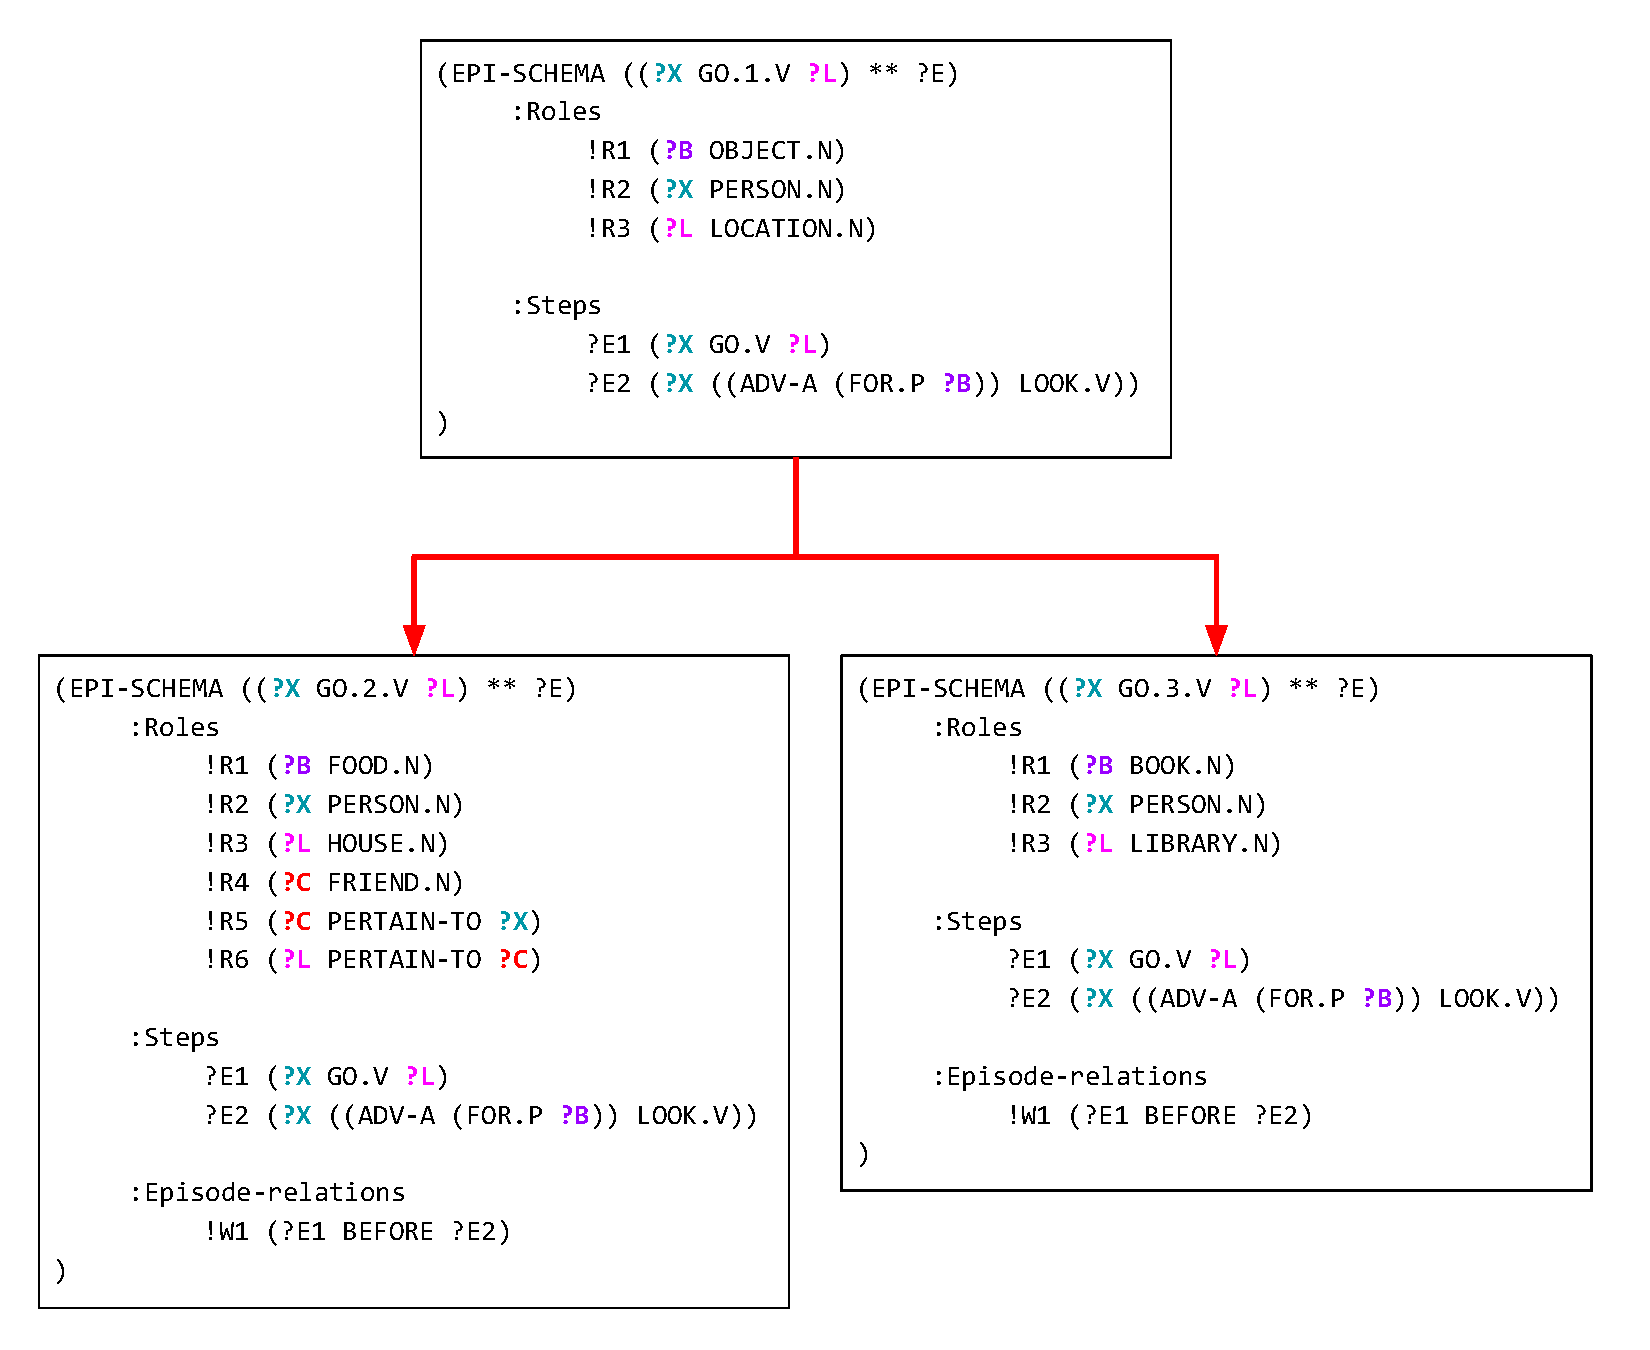
\includegraphics[width=\columnwidth]{CH3_schemas/inheritance}
    \caption{An illustration of the \textbf{specialization} hierarchy, in which two \textit{child} schemas inherit the semantics of a shared \textit{parent}.}
    \label{fig:spec_hier}
\end{figure}